
\documentclass[tikz,border=8pt]{standalone}
\usepackage{amsmath}
\usepackage{xcolor}
\usetikzlibrary{arrows.meta,positioning,calc,shapes.geometric}
\definecolor{Canvas}{HTML}{FAF9F6}
\definecolor{Ivory}{HTML}{FFFFF0}
\definecolor{Divider}{HTML}{E5E5EA}
\definecolor{Gold}{HTML}{C5A059}
\definecolor{WarmGold}{HTML}{D4AF37}
\definecolor{SoftPink}{HTML}{FBEFEF}
\definecolor{Ink}{HTML}{2C2C2E}
\tikzset{decision/.style={rectangle,draw=Gold,line width=1.2pt,fill=Canvas,minimum width=1.5cm,minimum height=1cm,align=center,text=Ink},chance/.style={circle,draw=WarmGold,line width=1.2pt,fill=Ivory,minimum size=1.45cm,align=center,text=Ink},payoff/.style={regular polygon,regular polygon sides=3,shape border rotate=90,draw=Gold,line width=1.2pt,fill=SoftPink,minimum size=1.25cm,align=center,text=Ink},branch/.style={draw=Ink,line width=0.9pt,-{Latex[length=2mm]},line cap=round},chosenbranch/.style={draw=Gold,line width=1.15pt,-{Latex[length=2mm]},line cap=round},callout/.style={rectangle,rounded corners=5pt,draw=Divider,fill=Ivory,text=Ink,align=center,inner sep=6pt}}

% Asset ID: OffSpecDecisionAnalysisTikZ-003
% Source: transcripts.md, Jess two-dice and third-die worked example
% Purpose: Show Jess's multi-stage decision tree and backward EMV logic.
\begin{document}
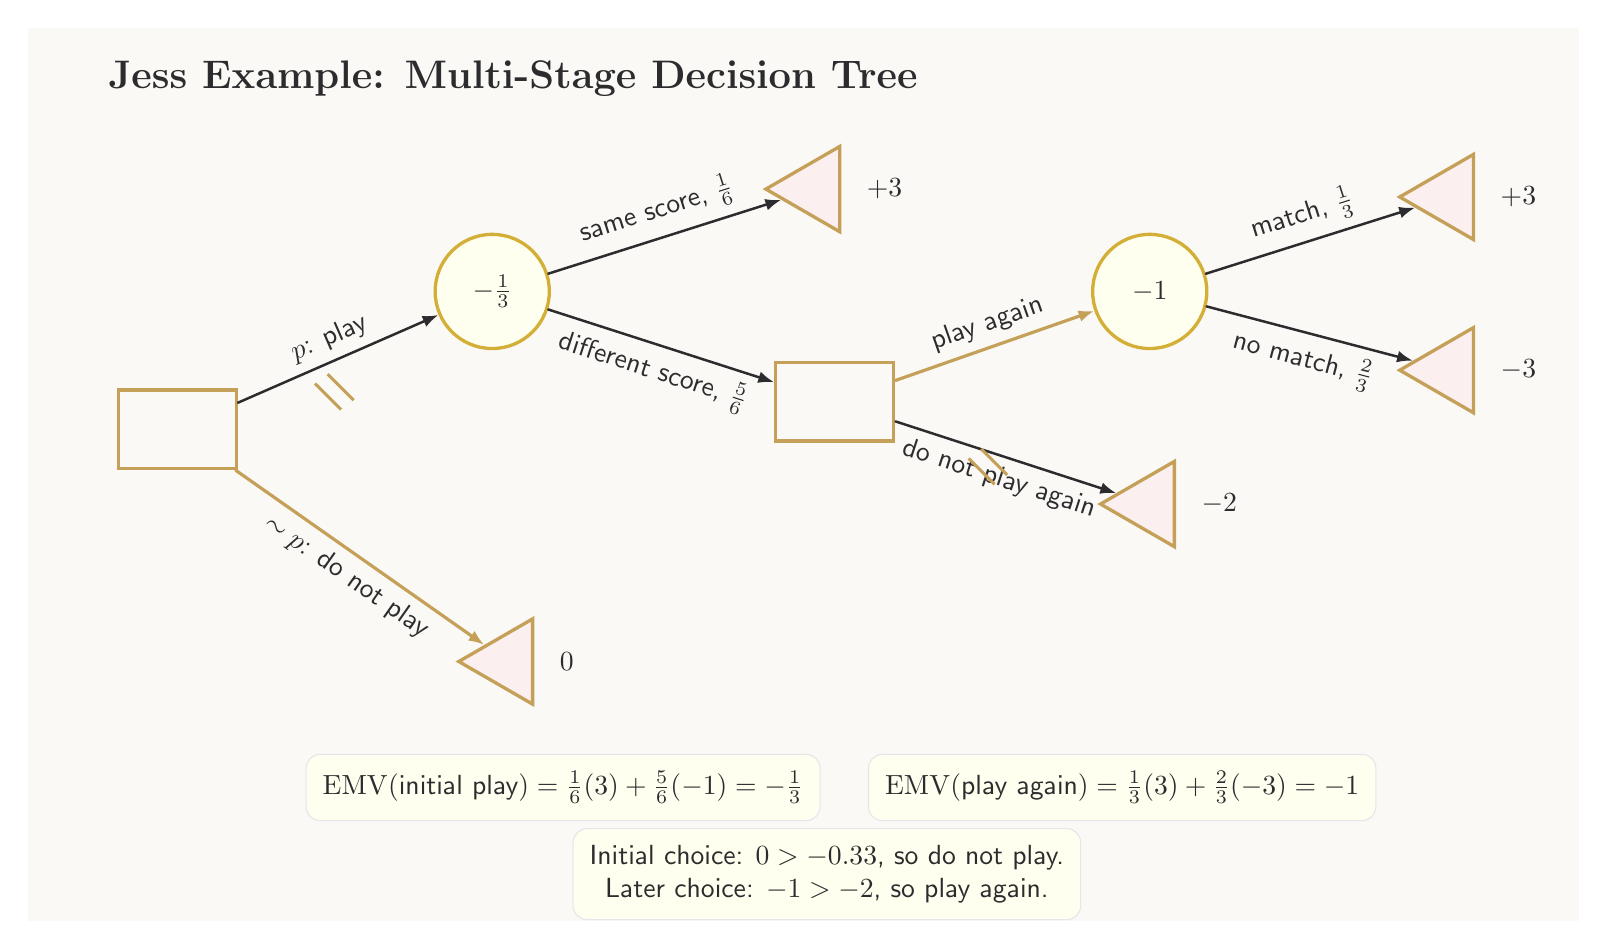
\begin{tikzpicture}[font=\sffamily,x=1cm,y=1cm]
\fill[Canvas] (-0.9,-2.25) rectangle (18.8,9.1);
\node[anchor=west,text=Ink,font=\bfseries\Large] at (0,8.45) {Jess Example: Multi-Stage Decision Tree};
\node[decision] (D0) at (1.0,4.0) {};\node[chance] (C1) at (5.0,5.75) {$-\frac13$};\node[payoff] (Same) at (9.1,7.05) {};\node[decision] (D2) at (9.35,4.35) {};\node[payoff] (NoPlay) at (5.2,1.05) {};\node[chance] (C2) at (13.35,5.75) {$-1$};\node[payoff] (Stop) at (13.35,3.05) {};\node[payoff] (Match) at (17.15,6.95) {};\node[payoff] (NoMatch) at (17.15,4.75) {};
\draw[branch] (D0)--node[above,sloped,text=Ink] {$p$: play} (C1);\draw[chosenbranch] (D0)--node[below,sloped,text=Ink] {$\sim p$: do not play} (NoPlay);
\draw[Gold,line width=1.1pt] (2.75,4.58)--(3.08,4.25);\draw[Gold,line width=1.1pt] (2.91,4.70)--(3.24,4.37);
\draw[branch] (C1)--node[above,sloped,text=Ink] {same score, $\frac16$} (Same);\draw[branch] (C1)--node[below,sloped,text=Ink] {different score, $\frac56$} (D2);
\draw[chosenbranch] (D2)--node[above,sloped,text=Ink] {play again} (C2);\draw[branch] (D2)--node[below,sloped,text=Ink] {do not play again} (Stop);
\draw[Gold,line width=1.1pt] (11.05,3.63)--(11.38,3.30);\draw[Gold,line width=1.1pt] (11.21,3.75)--(11.54,3.42);
\draw[branch] (C2)--node[above,sloped,text=Ink] {match, $\frac13$} (Match);\draw[branch] (C2)--node[below,sloped,text=Ink] {no match, $\frac23$} (NoMatch);
\node[anchor=west,text=Ink] at ($(Same.east)+(0.20,0)$) {$+3$};\node[anchor=west,text=Ink] at ($(NoPlay.east)+(0.20,0)$) {$0$};\node[anchor=west,text=Ink] at ($(Stop.east)+(0.20,0)$) {$-2$};\node[anchor=west,text=Ink] at ($(Match.east)+(0.20,0)$) {$+3$};\node[anchor=west,text=Ink] at ($(NoMatch.east)+(0.20,0)$) {$-3$};
\node[callout] at (5.9,-0.55) {$\operatorname{EMV}(\text{initial play})=\frac16(3)+\frac56(-1)=-\frac13$};
\node[callout] at (13.0,-0.55) {$\operatorname{EMV}(\text{play again})=\frac13(3)+\frac23(-3)=-1$};
\node[callout] at (9.25,-1.65) {Initial choice: $0>-0.33$, so do not play.\\Later choice: $-1>-2$, so play again.};
\end{tikzpicture}
\end{document}
